\scanpage{45}
On pourra donc poser
\[
\eta_s=\xi_s T_\nu^{\delta_\nu}T_{\nu+1}^{\delta_{\nu+1}}\cdots T_{r-1}^{\delta_{r-1}}(T_r,\cdots T_{s-1})^{p-1}
\]
avec $\xi_s\in M$

On aura
\[
\eta_sT_s^{p-1}=\xi_sT_\nu^{\delta_\nu}\cdots T_{r-1}^{\delta_{r-1}}(T_r\cdots T_s)^{p-1}
\]
Et relation $(R_s)$ s'écrit donc, comme
\[
p\nu'_s\eta_{s+1}=\unsure{(p\nu'_s)}\xi_{s+1}T_\nu^{\delta_\nu}\cdots T_{r-1}^{\delta_{r-1}}(T_r\cdots T_s)^{p-1}
\]
\[
\boxed{\xi_s=p\nu'_s\xi_{s+1}}
\]
On aura donc
\[
\xi_s=p^h\nu'_s\cdots\nu'_{s+h-1}\xi_{s+h}\qquad\forall h\geq1
\]
donc
\[
\xi_s\in\deleted{\unsure{\varphi}}\bigcap_h(p^hM)
\]
i.e. les $\xi_s$ appartiennent à la partie divisible de $\uline{M}$.
\figure{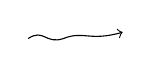
\begin{tikzpicture}\draw[->] (0,0)..controls(.2,.13)and(.22,-.08)..(.45,0)..controls(.7,.1)and(.78,-.04)..(1.2,.08);\end{tikzpicture}}

\uline{Prop} Soit $k$ un anneau comm., $\unsure{S_k|B_k}=k\{T\}$, $M,N$ deux $k$-modules, avec $d>0$, $N_0^{\unsure{?|*}}=\bigcap_{n\in\mathbb N^*}nN$ le \deleted{partie} \inserted{plus grand sous-module} divisible de $N$, $\alpha\geq d$. Alors si $u\in\operatorname{Hom}^{-d}(\tau_\alpha M_{S_k},N_{S_k})$ (\deleted{qui} \inserted{lequel module} est indépendant \unsure{mod variation} du choix de $\alpha$), $u$ se factorise par $N_{0S_k}$, i.e.
\[
\operatorname{Hom}^{-d}(\tau_\alpha M_{S_k},N_{S_k})\overset{\sim}{\longleftrightarrow}\operatorname{Hom}^{-d}(\tau_\alpha M_{S_k},N_{0S_k})
\]
\uline{Cor} Si $N_0=0$, p. ex. $k$ de torsion, alors $\operatorname{Hom}^{-d}(\tau_\alpha M_{S_k},N_{S_k})=0$
\mspage{44}
